A robust estimate of the basis vector is crucial for developing a trading
strategy with any confidence. While the Johansen procedure is very efficient
and produces good estimates in theory, the time series used in practice are
often very noisy and have periods of intermittent cointegration (structural
breaks) which can damage our overall estimate of the relationship. To improve
our estimate we use a system of ``weak'' experts and combine them to form
robust basis vector with, empirically speaking, much better convergence
properties.

The weak estimators are formed by applying the Johansen procedure over varying
data slices, such as a moving window for using the entire observed dataset up
to time $t$. One may then apply smoothing, such as (exponentially-weighted)
moving averages or Bayesian parameter estimation procedures, on top of this to
further improve robustness of each individual expert.

\section{Normal-Normal model}
We consider a univariate Gaussian model for the observed values of the basis
vector, $\mathcal{N}(\mu, \sigma^2)$, in which the variance is assumed known
but the mean is estimated. We let $D = (x_1, \ldots, x_n)$ be the data such
that the likelihood takes the form,
\begin{align}
    p(D \mid \mu, \sigma^2) &= \prod_{i=1}^n p(x_i \mid \mu, \sigma^2), \\
    &= (2\pi\sigma^2)^{-n/2}
           \exp\left[-\frac{1}{2\sigma^2} \sum_{i=1}^n (x_i - \mu)^2\right].
\end{align}
Assuming a constant $\sigma^2$, we have the following relationship,
\begin{align}
    p(D \mid \mu, \sigma^2) &\propto
        \exp\left[-\frac{n}{2\sigma^2}(\bar x - \mu)^2\right], \\
    &\propto \mathcal{N}(\bar x \mid \mu, \frac{\sigma^2}{n}).
\end{align}

For simplicity, we use the natural conjugate prior for $p(\mu) \propto
\mathcal{N}(\mu \mid \mu_0, \sigma_0^2)$ to obtain nice closed-form solutions
for the estimate updates. After some simple manipulation one obtains the following update rules:
\begin{align}
    \sigma_n^2 &= \frac{\sigma^2\sigma_0^2}{n\sigma_0^2 + \sigma^2}, \\
    \mu_n &= \sigma_n^2\left(\frac{\mu_0}{\sigma_0^2} + \frac{n\bar
        x}{\sigma^2}\right).
\end{align}

\subsection{Good priors}
It's important that a good prior, $p(\mu)$, is used in order to get an
practicable estimation of the basis early on. To do this, we look at the
historical distributions of basis vectors (Tab.~\ref{tab:bbprior}) and assume
that they are indicative of future relationships. For completeness, we include
the distributions for different periods of each match, where $\mu_0$ and
$\sigma_0$ are the mean and standard deviation on the prior, respectively.
\begin{table}
    \centering
    \begin{tabular}{@{\textbf}lllll@{}}
        \toprule
        & $\mu_0$ & $\sigma_0$ & $m$    & $c$    \\
        \midrule
        Whole match    & 0.4920  & 0.0634     & 0.0024 & 0.4986 \\
        \midrule
        First quarter  & 0.4954  & 0.1188     & 0.0033 & 0.5067 \\
        Second quarter & 0.4950  & 0.1138     & 0.0038 & 0.4893 \\
        Third quarter  & 0.4890  & 0.1132     & 0.0035 & 0.4865 \\
        Fourth quarter & 0.4915  & 0.1121     & 0.0016 & 0.5000 \\
        \midrule
        First half     & 0.4925  & 0.0938     & 0.0031 & 0.4959 \\
        Second half    & 0.4922  & 0.0834     & 0.0028 & 0.5025 \\
        \bottomrule
    \end{tabular}

    \caption{Emprirical prior distributions over the cointegration basis vector
    of basketball team scores between 06/2015 to 11/2017.}\label{tab:bbprior}
\end{table}

To further improve our estimate we can consider the relationship between the
natural handicap on the match and the means of the given basis distributions.
The gradient, $m$, and intercept, $c$, may then be used to form an adjusted
estimate of $\mu_0$, given by the following,
\begin{equation}
    \mu_0 \sim m\cdot\textrm{NH} + c,
\end{equation}
where $\textrm{NH}$ is the natural handicap.

\section{Combining estimators}
Based on Gareth's voting scheme technical report, we used a minimum variance
estimator (MVE) to combine the weak experts. This assumes that the individual
estimates are unbiased, which is likely untrue, but forms a decent first method
for combining in a single unbiased strong estimator. In practice one may know a
priori that some estimators should be weighted higher but we leave this is for
future work.

The MVE estimator produces the following weights for a system of $K$
estimators,
\begin{equation}
    w_i = \frac{1/\sigma_i^2}{\sum_{k=1}^K(1/\sigma_k^2)},
\end{equation}
which yields a weighted average for the mean, with variance given by,
\begin{equation}
    \sigma^2 = \left(\sum_{k=1}^K \frac{1}{\sigma_k^2} \right)^{-1}.
\end{equation}


\section{Case Study}
To illustrate the effectiveness of the MVE estimator, we present an
example\footnote{Note that the results do carry across matches, this is not
just a one off.} using a basketball match between the Dallas Mavericks and the
New York Knicks.

\begin{figure}[H]
    \centering
    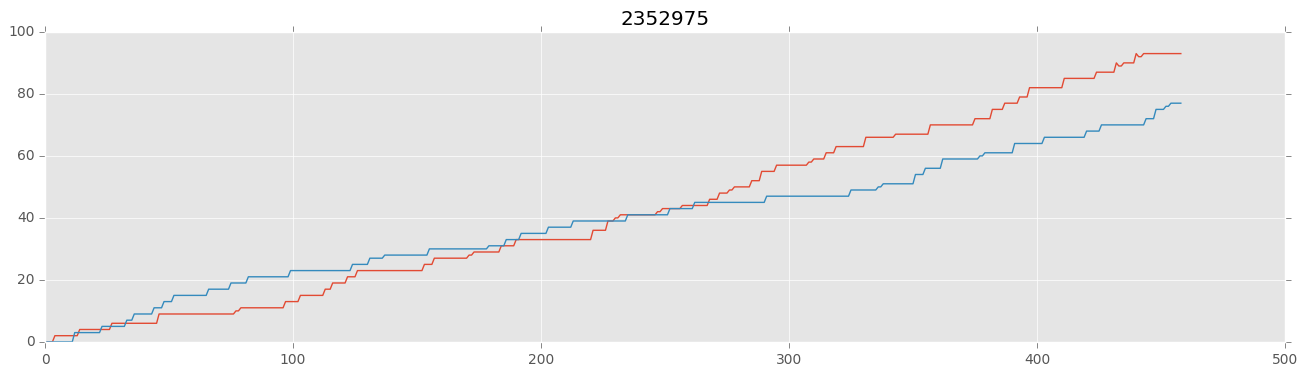
\includegraphics[width=\figwidth]{img/estimation/scores.png}

    \caption{Scores of teams A (red) and B (blue) for the basketball match with
    event id 2352975.}\label{fig:estimation:scores}
\end{figure}

\begin{figure}[H]
    \begin{subfigure}[b]{0.49\textwidth}
        \centering
        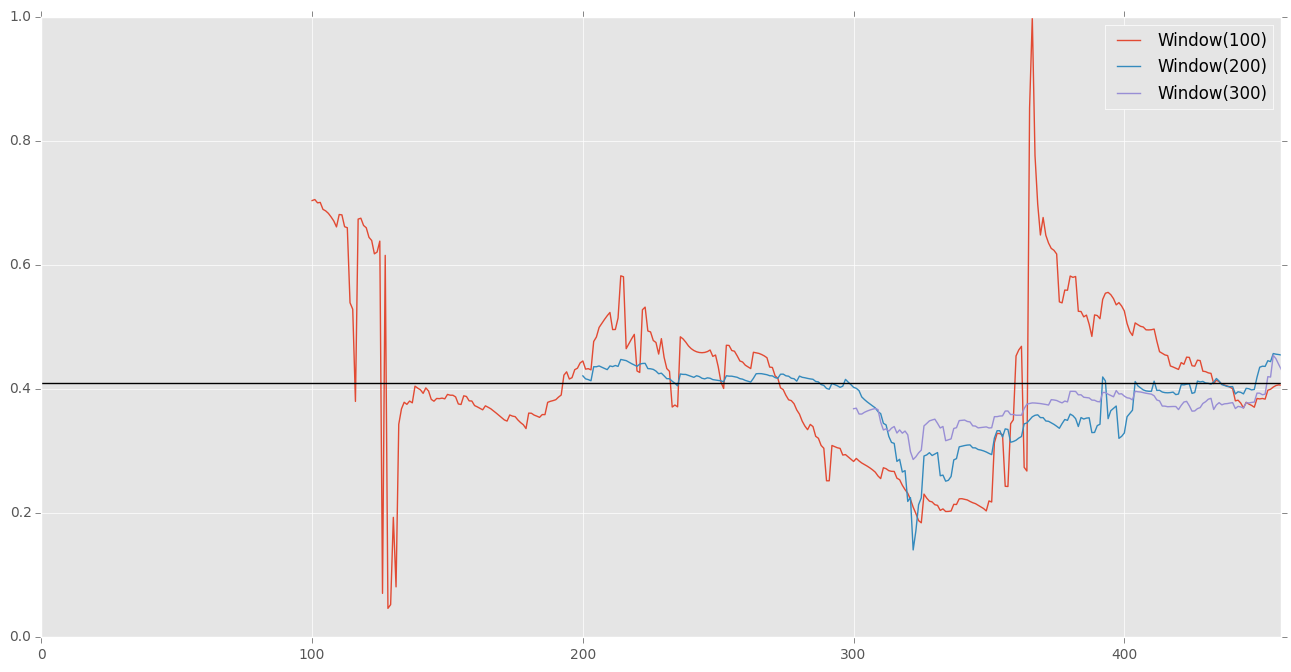
\includegraphics[width=\figwidth]{img/estimation/windowed_raw.png}

        \caption{Raw}
    \end{subfigure}
    \hfill
    \begin{subfigure}[b]{0.49\textwidth}
        \centering
        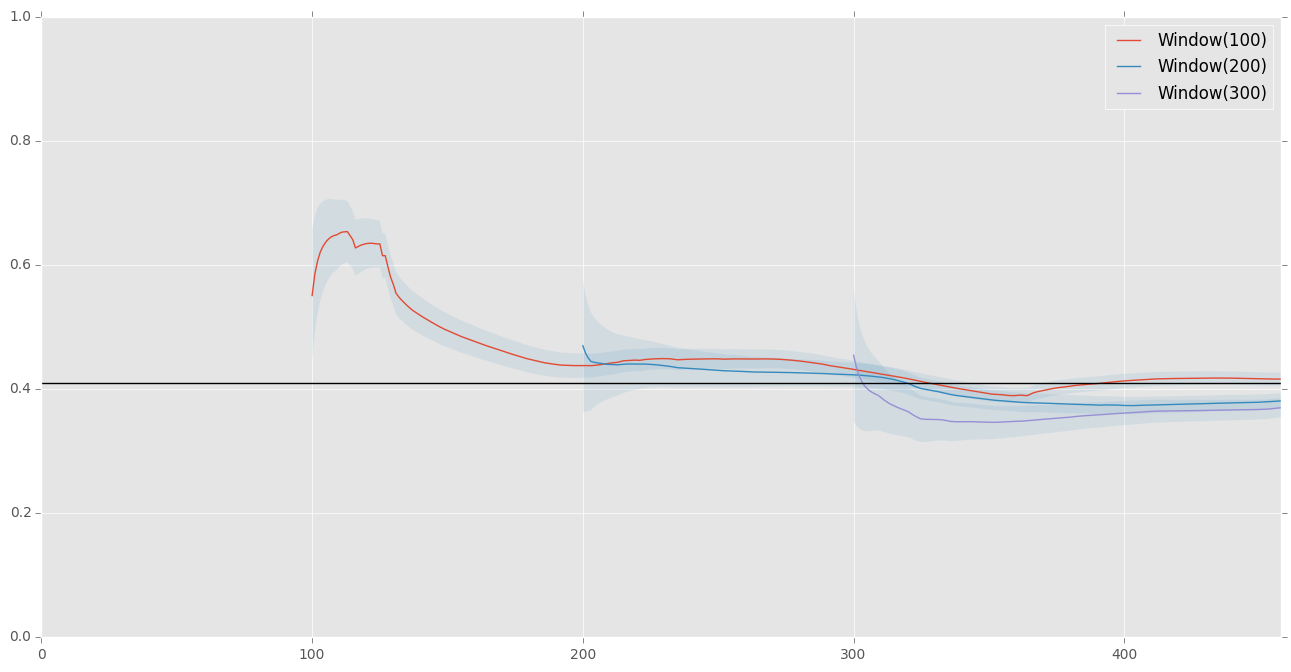
\includegraphics[width=\figwidth]{img/estimation/windowed_bayes.png}

        \caption{Bayes}
    \end{subfigure}

    \caption{Estimations of the cointegration basis (first component) given
    using a moving window.}\label{fig:estimation:windowed}
\end{figure}

\begin{figure}[H]
    \begin{subfigure}[b]{1.0\textwidth}
        \centering
        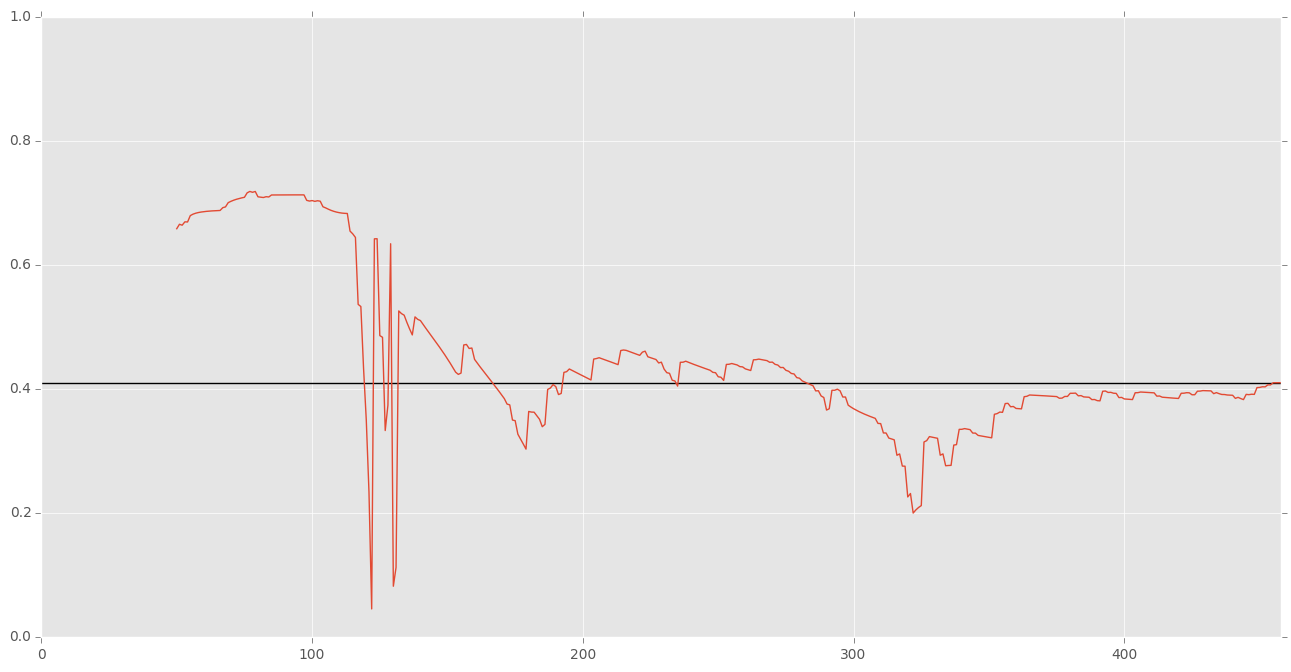
\includegraphics[width=\figwidth]{img/estimation/cumulative_raw.png}

        \caption{Raw}
    \end{subfigure}
    \\[1em]
    \begin{subfigure}[b]{0.49\textwidth}
        \centering
        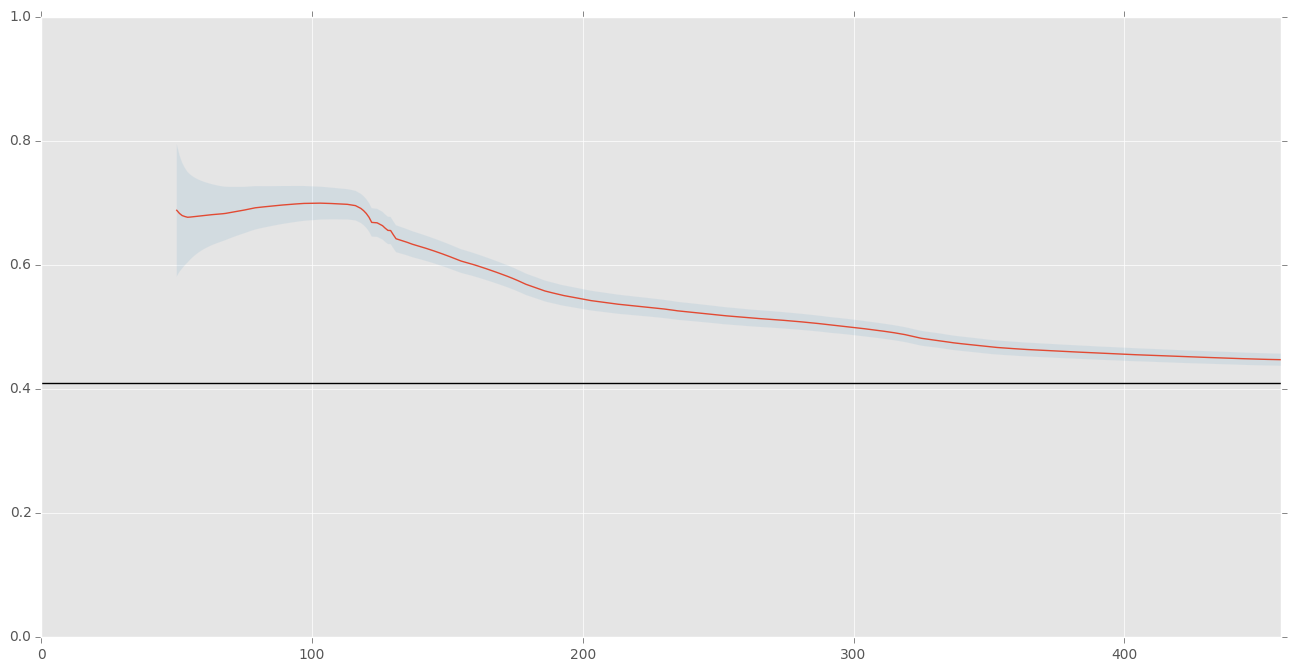
\includegraphics[width=\figwidth]{img/estimation/cumulative_bayes.png}

        \caption{Bayes}
    \end{subfigure}
    \hfill
    \begin{subfigure}[b]{0.49\textwidth}
        \centering
        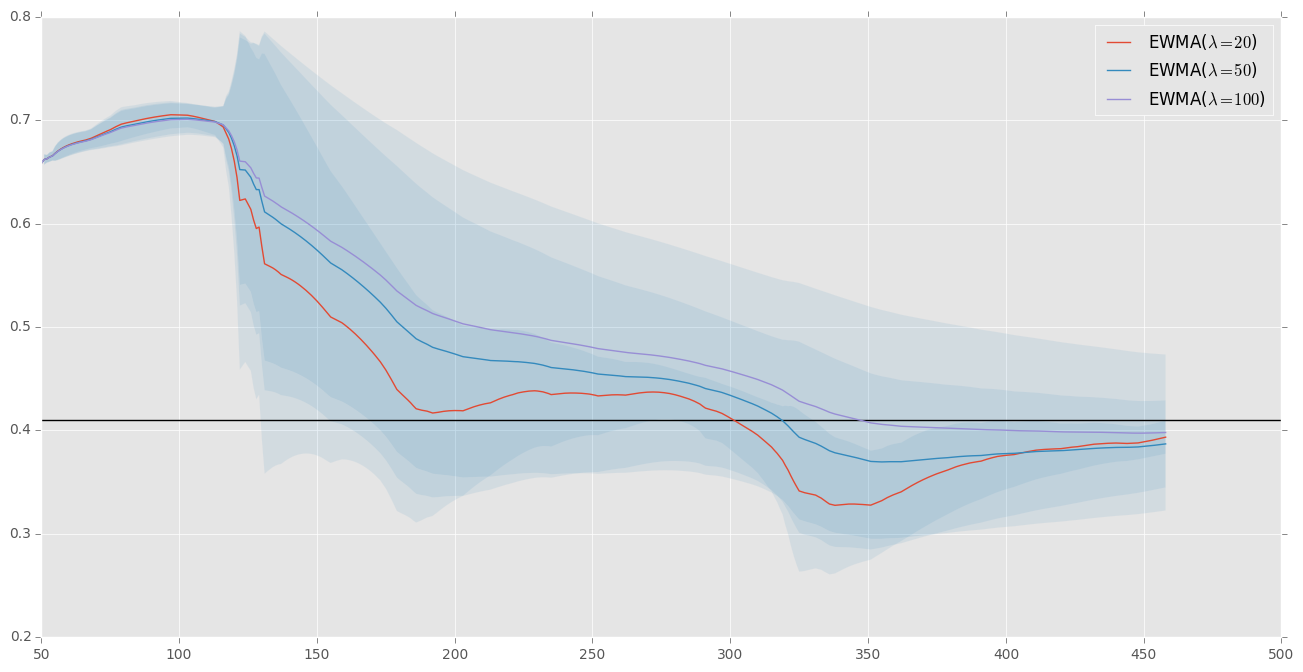
\includegraphics[width=\figwidth]{img/estimation/cumulative_ewma.png}

        \caption{Exponentially-weighted moving average}
    \end{subfigure}

    \caption{Estimations of the cointegration basis (first component) given
    using an accumulated window of all observed
    estimations.}\label{fig:estimation:cumulative}
\end{figure}

\begin{figure}[H]
    \centering
    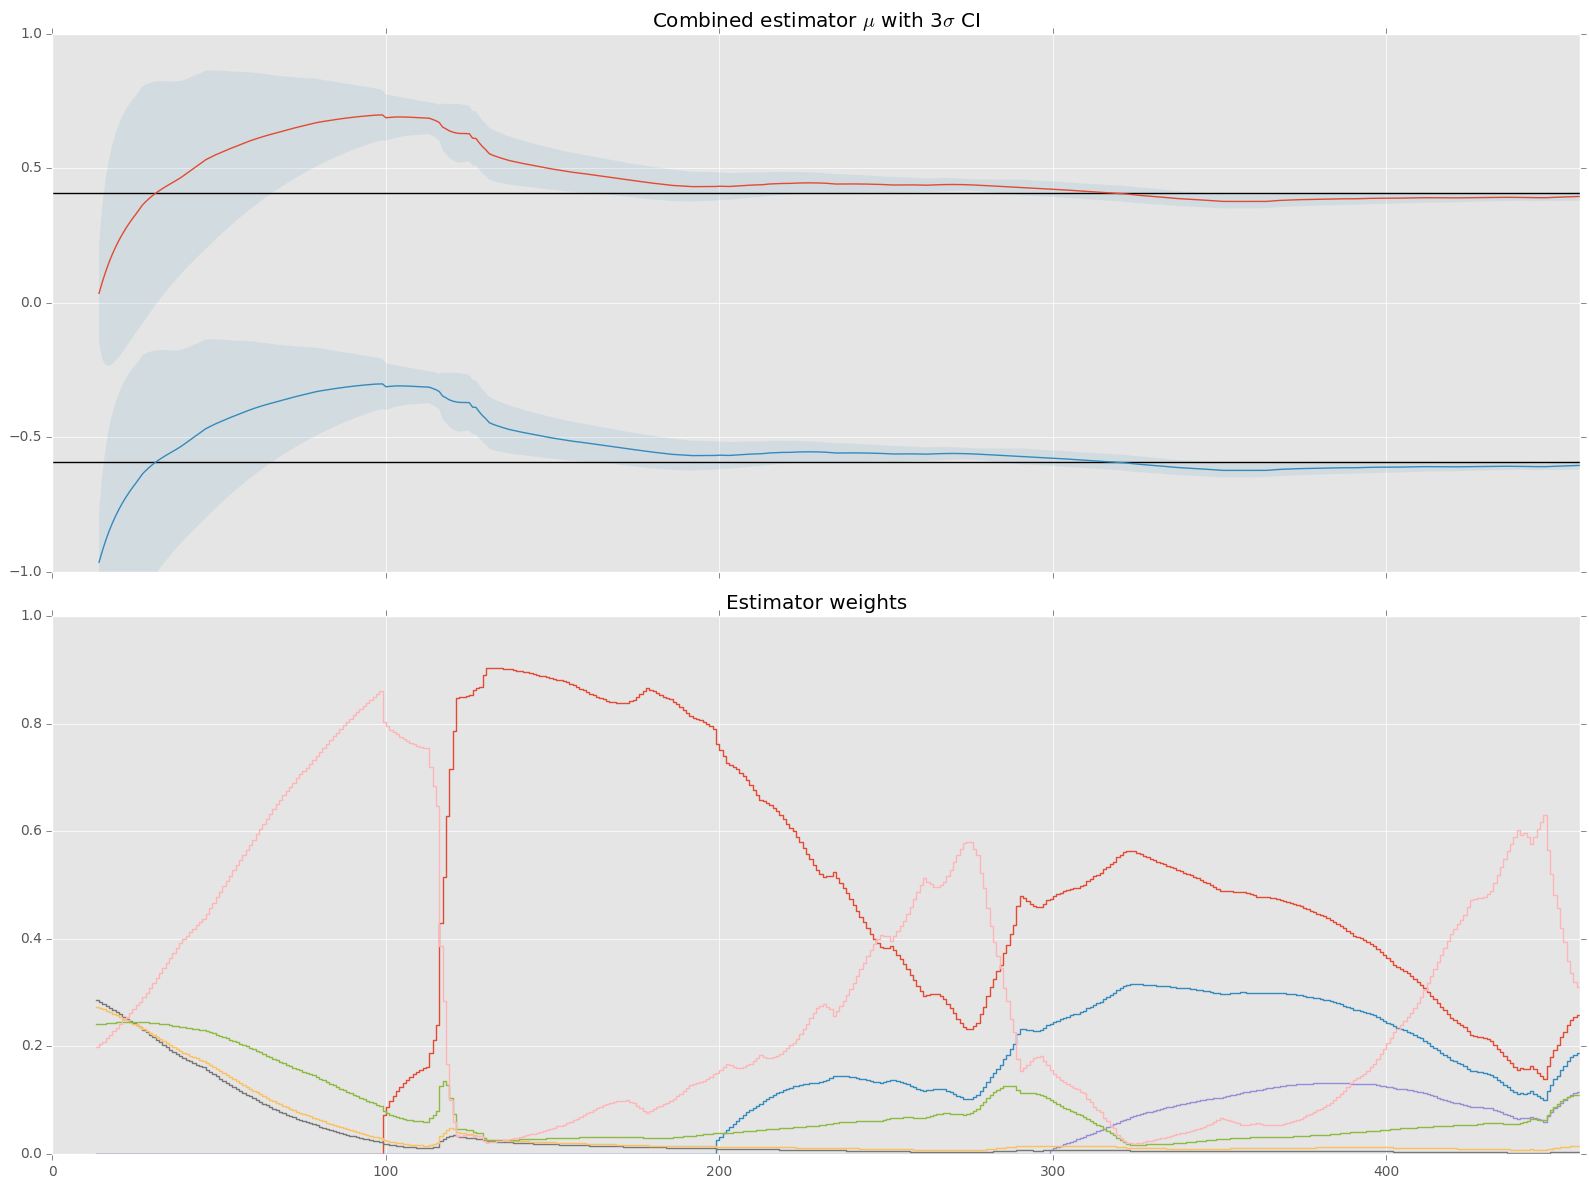
\includegraphics[width=\figwidth]{img/estimation/mve.png}

    \caption{Minimum variance estimation of the cointegration basis using a
    combination of Bayesian windowed estimators and exponentially-weighted
    moving average cumulative estimators.}\label{fig:estimation:mve}
\end{figure}

\begin{figure}[H]
    \centering
    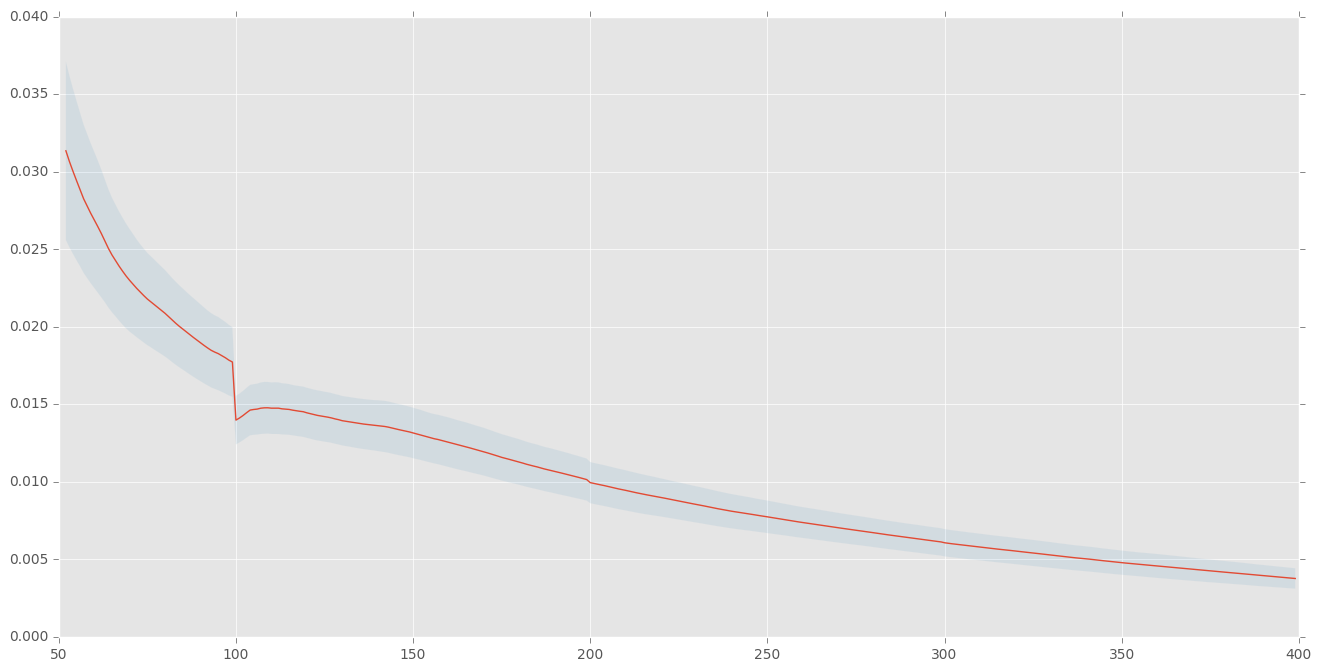
\includegraphics[width=\figwidth]{img/estimation/mse.png}

    \caption{Distribution of the mean squared error of the estimation against
    the best estimate across all recorded matches in the period 06/2015 to
    11/2017. The mean (red line) is quoted along with the $3\sigma$ confidence
    interval.}\label{fig:estimation:mse}
\end{figure}
